\documentclass{PPFIT} % pro psaní v angličtině / for writing in English
%\documentclass[czech]{PPFIT} % pro psaní v češtině / for writing in Czech
%\documentclass[slovak]{PPFIT} % pro psaní ve slovenštině / for writing in Slovak

%--------------------------------------------------------
%--------------------------------------------------------
%	PŘIZPŮSOBENÍ PDF / PDF CUSTOMIZATION
%--------------------------------------------------------
\usepackage{amsthm}
\usepackage{amssymb}
\usepackage{stfloats}
\usepackage{tikz}
\usetikzlibrary{shapes,shapes.geometric,arrows,fit,calc,automata,positioning}
\tikzset{elliptic state/.style={draw, ellipse, inner sep=1mm}}
\tikzset{rectangular state/.style={draw, rounded rectangle, inner sep=2mm, minimum height=0.9cm}}
\usepackage[ruled,vlined,linesnumbered,noresetcount]{algorithm2e}
\usepackage{lipsum}
\usepackage{caption}
\usepackage{subcaption}
\usepackage{multirow}

\hypersetup{
    pdftitle={Utilization of Repeating Substructures for Efficient Representation of Automata},
    pdfauthor={Bc. Michal Šedý},
    pdfkeywords={Nondeterministic Finite Automata, Minimization, Nondeterministic Pushdown Automata, Regular Expressions, Language Similarity}
}

%--------------------------------------------------------
%--------------------------------------------------------
%  PŘEDBĚŽNÁ vs. KONEČNÁ VERZE / REVIEW vs. FINAL VERSION
%--------------------------------------------------------
%   NECHTE následující řádek zakomentovaný pro PŘEDBĚŽNÉ VERZE
%   Pro KONEČNOU VERZI řádek odkomentujte.
%   LEAVE this line commented out for the REVIEW VERSIONS
%   UNCOMMENT this line to get the FINAL VERSION

\PPFinalCopy


\PPYear{2022/2023}

\ifczechslovak%
    %--------------------------------------------------------
    %--------------------------------------------------------
    %	INFORMACE O ČLÁNKU
    %--------------------------------------------------------

  \PaperTitle{Jak napsat skvělý článek}

    \Authors{Adam Herout*}
    \affiliation{*%
      \href{mailto:herout@fit.vut.cz}{herout@fit.vut.cz},
      \textit{Fakulta informačních technologií, Vysoké učení technické v Brně}}

    \Keywords{Klíčové slovo1 --- Klíčové slovo2 --- Klíčové slovo3}

    \Supplementary{\href{http://youtu.be/S3msCdn3fNM}{Demonstrační Video} --- \href{http://fit.vut.cz/}{Stáhnutelný Kód}}

    %--------------------------------------------------------
    %--------------------------------------------------------
    %	ABSTRAKT
    %--------------------------------------------------------
    \Abstract{
        \lipsum[1-2]
    }
\else%
    %--------------------------------------------------------
    %--------------------------------------------------------
    %	INFORMATION ABOUT THE ARTICLE
    %--------------------------------------------------------
    \PaperTitle{Utilization of Repeating Substructures for Efficient Representation of Automata}

    \Authors{Bc. Michal Šedý*}
    \affiliation{*%
        \href{mailto:xsedym02@stud.fit.vut.cz}{xsedym02@stud.fit.vut.cz},
        \textit{Faculty of Information Technology, Brno University of Technology}}

    \Keywords{Nondeterministic Finite Automata --- Minimization --- Nondeterministic Pushdown Automata --- Regular Expressions --- Language Similarity}

    % \Supplementary{\href{http://youtu.be/S3msCdn3fNM}{Demonstation video} --- \href{http://fit.vut.cz/}{Downloadable code}}

    %--------------------------------------------------------
    %--------------------------------------------------------
    %	ABSTRACT
    %--------------------------------------------------------
    \Abstract{
        Nondeterministic finite automata (NFA) are widely used across almost all fields of computer science, such as for a representation of regular expressions, monitoring high-speed networks, in abstract regular model checking, program verification, or in decision procedures of WS1S and WS2S logics. NFAs are even used in bioinformatics for searching sequences of nucleotides in DNA. The basic technique for reducing computational resources (memory, time, or the amount of hardware components) when working with NFAs is minimization. The most well-known minimization methods are state merging and transition pruning. Although combining these two methods can reduce the size of an automaton by up to 50\%, the resulting automaton can still contain duplicate (similar) transition sequences. There are even automata that cannot be minimized by these methods. This work presents a new way of automata minimization based on a transformation of a NFA into a~nondeterministic pushdown automaton (NPDA). The transformation identifies and represents the most similar parts (procedures) of the automaton only once. This algorithm enables the reduction of previously non-minimalizable automata and also improves the results of other minimizations. The principle of transforming NFA into NPDA can be understood as a transformation of a purely sequential program into a~program with mutually communicating procedures.
    }
\fi

%--------------------------------------------------------
%--------------------------------------------------------
%	TEASER
%--------------------------------------------------------
\Teaser{
%	\TeaserImage{placeholder.pdf}
%	\TeaserImage{placeholder.pdf}
%	\TeaserImage{placeholder.pdf}
}

%--------------------------------------------------------
%--------------------------------------------------------
%--------------------------------------------------------
%--------------------------------------------------------
\begin{document}
\startdocument
%--------------------------------------------------------
%--------------------------------------------------------
%	OBSAH ČLÁNKU / CONTENT OF THE ARTICLE
%--------------------------------------------------------
\ifczechslovak
    % \input{2023-xsedym02-text.tex}
\else
    \section{Introduction}

    Nondeterministic finite automata (NFA) were introduced by Michael Rabin and Dana Scott in \cite{FA_and_Their_Decisin_Problems}. Unlike their deterministic counterpart, NFAs have the ability to make a transition to multiple states based on the same input symbol. This allows NFAs to represent the language more compactly. However, this feature makes the minimization of NFAs difficult. Despite the difficulty of minimization, NFAs are widely used in almost all fields of computer science, such as representing regular expressions, monitoring high-speed networks \cite{FPGA_based_network_scaning}, in abstract regular model checking \cite{ARMC}, in verifying programs that manipulate strings \cite{String_constraints_for_ver} or in decision procedures in the WS1S and WS2S logic \cite{On_equivalence_checking, Nested_antichains_for_WS1S}. NFAs are even used in bioinformatics to search for nucleotide sequences in DNA \cite{DNA_pattern_analysis_using_FA}.

    The basic technique for reducing computational requirements when working with NFA is minimization. The most well-known minimization technique is a state merging \cite{Oldest_Merge,Simulation_based_minimization,On_nfa_reduction}, which searches for two language equivalent states and then merges them into one. Another approach is transition pruning \cite{Simulation_based_minimization, Lorenzo_prunning_saturation}, which removes transitions from the state with weaker language based on language inclusion. The opposite of transition pruning is transition adding (saturation) \cite{Oldest_Merge, Lorenzo_prunning_saturation}, where newly added transitions may allow further state merging or transition pruning.

    The mentioned minimization methods reduce the size of most automata by up to 50\%, but duplicitous transition sequences still exist in the resulting automata. There are also types of automata that cannot be minimized by current methods, such as automata with a~linear structure (without branching) or automata representing words with a given infix, same prefix, and suffix (e.g. \textit{abba, cbbc}). In these cases, state merging, transition pruning, and saturation cannot minimize the automata, because these reduction methods are based on language inclusions and these types of automata do not contain any. In the structure of these automata, only similar transition segments occur (e.g. \textit{bb} from the previous example).


    This work describes a new minimization algorithm that uses the similarity of transition sequences in order to reduce the size of the automaton. The approach involves the informed conversion of a nondeterministic finite automaton (NFA) to a nondeterministic pushdown automaton (NPDA). In the NPDA, similar sequences can be replaced by one procedure that uses the symbol stored on the stack to determine the branch of the original automaton where the calculation is located. The goal of a successful transformation is to replace such sequences of transitions that the savings from their reduction will exceed the overhead of the stack operations. The reduction of automata representing regular expressions can be improved on average by 32.1\% using this minimization approach.

    The transformation of NFA to NPDA can be understood as the conversion of a purely sequential program to a program using communicating procedures. Like the NPDA, a call stack is used in the program to maintain information about the current branch and where the calculation should return to after the procedure ends.

\section{Preliminaries}
    This section defines the fundamental terms utilized in our reduction approach, such as nondeterministic finite automaton, nondeterministic push down automaton. Additionally, it introduces the simulation relation and the product of a NPDA, which represents all possible procedure candidates.

    \subsection{Nondeterministic Finite Automaton}
        A \textit{Nondeterministic Finite Automaton} (NFA) is a 5-tuple $M = (Q, \Sigma, \delta, I, F)$, where:
        \begin{itemize}
            \item $Q$ is a finite set of states,
            \item $\Sigma$ is an alphabet,
            \item $\delta : Q \times \Sigma \rightarrow 2^Q$ is a transition function,
            \item $I \subseteq Q$ is a set of initial states, and
            \item $F \subseteq Q$ is a set of final states.
        \end{itemize}

        The transition function $\delta$ can be generalized for a~set of symbols. Let $q \in Q$ and $A \subseteq \Sigma$, then $\delta(q, A) = \bigcup_{a\in A} \delta(q, a)$.

        We also define the inverse function $\delta^{-1}$, where: $q \in \delta^{-1}(r, a) \iff r \in \delta(q, a)$, for $a \in \Sigma$ and $q, r \in Q$.

        \subsubsection*{Configuration}
            A \textit{configuration} of a NFA is an ordered pair $C \in Q \times \Sigma^*$. $(q, w) \in C$ indicates that the automaton is in state $q$ and that the unprocessed string $w$ remains on the input.

        \subsubsection*{Transition}
            A \textit{transition} is a binary relation $\vdash\, \subseteq C \times C$, defined as follows: $(q, w) \vdash (r, w') \iff w = aw' \land r \in \delta(q, a)$, for $q, r \in Q$, $w, w' \in \Sigma^*$, $a \in \Sigma$.

        \subsubsection*{Language}
            The \textit{forward language} of state $q \in Q$ is the set $\overrightarrow L(q) = \{w \in \Sigma^*\,|\, (q, w) \vdash (f, \epsilon)\textnormal{, where }f \in F\}$.

            The \textit{backward language} of state $q \in Q$ is the set $\overleftarrow L(q) = \{w \in \Sigma^*\, |\, (i, w) \vdash (q, \epsilon)\textnormal{, where }i \in I\}$.

            The \textit{language of the automaton} $M$ is the set defined as $L(M)=\bigcup_{i \in I} \overrightarrow L(i)$.


    \subsection{Nondeterministic Pushdown Automaton}
        A \textit{Nondeterministic Pushdown Automaton} (NPDA) is an 8-tuple $M = (Q, \Sigma_\epsilon, \Gamma_\epsilon, \delta, I, \lambda, F, \phi)$, where:
        \begin{itemize}
            \item $Q$ is a finite set of states,
            \item $\Sigma_\epsilon$ is an alphabet containing symbol $\epsilon$,
            \item $\Gamma_\epsilon$ is a stack alphabet containing symbol $\epsilon$,
            \item $\delta : Q \times \Sigma_\epsilon \times \Gamma_\epsilon \rightarrow 2^{Q \times \Gamma_\epsilon}$ is a transition function,
            \item $I \subseteq Q$ is a set of initial states,
            \item $\lambda: I \rightarrow 2^{\Gamma_\epsilon} \setminus \{\emptyset\}$ is a function of initial stack symbols,
            \item $F \subseteq Q$ is a set of final states, and
            \item $\phi: F \rightarrow 2^{\Gamma_\epsilon} \setminus \{\emptyset\}$ is a function of final stack symbols.
        \end{itemize}

        The function $\lambda$ specifies the initial stack symbol for an initial state. Let $i \in I$. If $\lambda(i) = \{\epsilon\}$, then the automaton starts in state $i$ with an empty stack. On the other hand, if $\lambda(i) = G \neq \{\epsilon\}$, then the automaton can start in state $i$ with a nondeterministically chosen symbol from set $G$.

        The function $\phi$ specifies the acceptance combination of a state and a stack symbol. Let $f \in F$. If $\phi(f) = \{\epsilon\}$, then the automaton accepts in state $f$ with an empty stack. Conversely, if $\phi(f) = G \neq \{\epsilon\}$, then the automaton accepts in state $f$ if the symbol $g$ on the top of the stack belongs to set $G$.

        Similarly to NFA, a transition function can also be defined for a set of symbols $A \subseteq \Sigma_\epsilon$ or $B \subseteq \Gamma_\epsilon$.

        The inverse transition function $\delta^{-1}$ of NPDA, is defined as: $(q, \beta) \in \delta^{-1}(r, a, \gamma) \iff (r, \gamma) \in \delta(q, a, \beta)$, where $q,r \in Q$, $a \in \Sigma_\epsilon$, $\beta, \gamma \in \Gamma_\epsilon$. Note that in the inverse transition function, the push and pop stack symbols are swapped.

        \subsubsection*{Configuration}
            A \textit{configuration} of a NFA is an ordered triple $C \in Q \times \Sigma^* \times \Gamma^*$, where $(q, w, \beta) \in C$ means that the machine is in the state $q$, the remaining unprocessed string is $w$, and the stack contains the string $\beta$ (the top of the stack is on the left).

        \subsubsection*{Transition}
            A \textit{transition} is a binary relation $\vdash\, \subseteq C \times C$, where: $(q, w, \beta) \vdash (r, w', \beta') \iff w = aw' \land \beta = X\alpha \land \beta' = Y\alpha \land (r, Y) \in \delta(q, a, X)$, for $q, r \in Q$, $w, w' \in \Sigma^*$, $a \in \Sigma_\epsilon$, $X, Y \in \Gamma_\epsilon$.

        \subsubsection*{Language}
            A \textit{forward language} of state $q \in Q$ with a stack $\alpha \in \Gamma^*$ is a set $\overrightarrow L(q, \alpha) = \{w \in \Sigma^*\, |\, (q, w, \alpha) \vdash (f, \epsilon, \beta) \land \beta \in \phi(f)\textnormal{, where }\beta \in \Gamma_\epsilon, f \in F\}$.

            A \textit{language of the automaton} $M$ is the set defined as $L(M)=\bigcup_{i \in I} \bigcup_{\alpha \in \lambda(i)} \overrightarrow L(i, \alpha)$.

        \subsubsection*{Transition Alphabet}
            \textit{Transition Alphabet} of a transition between states $q$ and $r$ from $Q$ is a set $\sigma(q, r) = \{a \in \Sigma\,|\, \exists \alpha, \beta \in \Gamma_\epsilon: (r, \beta) \in \delta(q, a, \alpha)\}$. It is the set of symbols from $\Sigma$ that label the transitions from state $q$ to state $r$.

            \textit{Epsilon Transition Alphabet} of a transition between states $q$ and $r$ from $Q$ is a set $\sigma_\epsilon(q, r) = \{a \in \Sigma\,|\, (r, \epsilon) \in \delta(q, a, \epsilon)\}$. For each symbol in this set, there exists a transition that goes from state $q$ to $r$ without access the stack.

            \textit{Nonepsion Transition Alphabet} of a transition between states $q$ and $r$ from $Q$ is a set $\overline{\sigma_\epsilon}(q, r) = \sigma(q, r) \setminus \sigma_\epsilon(q, r)$. It is a complement of the Epsilon Transition Alphabet.

        \subsubsection*{Stack Alphabet of State}
            \textit{Stack Alphabet of State} $q \in Q$ is a set $\gamma(q) = \{\alpha \in \Gamma \setminus \{\epsilon\}\,|\,(i, w, \beta) \vdash^* (r, w', \alpha\beta')\textnormal{, where }i \in I, r \in Q, w, w' \in \Sigma^*, \beta \in \lambda(i), \beta' \in \Gamma^*\}$. It is a set of stack symbols that can appear on the top of the stack while the automaton is in the state $q$.

    \subsection{Representation of NFA using NPDA}
        \label{sec:NFAasNPDA}
        The conversion of a NFA to its language equivalent NPDA is the initial step in our reduction approach that employs procedure mapping, and it is carried out as follows.

        Fore every NFA $M_{F} = (Q_{F}, \Sigma_{F}, \delta_{F}, I_{F}, F_{F})$ there exists its language equivalent $((M_{F}) \equiv L(M_{P}))$ NPDA $M_{P} = (Q_{P},\, \Sigma_{P}, \Gamma_\epsilon, \delta_{P}, I_{P}, \lambda, F_{P}, \phi)$, where:
            \begin{itemize}
                \item $Q_{P} = Q_{F}$,
                \item $\Sigma_{P} = \Sigma_{F}$,
                \item $\Gamma_\epsilon = \{\epsilon\}$,
                \item $\delta_{P}(q, a, \epsilon) = \delta_{F}(q, a) \times \{\epsilon\}$ for $q \in Q_{P}, a \in \Sigma_{P}$,
                \item $I_{P} = I_{F}$,
                \item $\lambda(i) = \{\epsilon\}$ for $i \in I$,
                \item $F_{P} = F_{F}$, and
                \item $\phi(f) = \{\epsilon\}$ for $f \in F$.
            \end{itemize}

        In this work, only nondeterministic pushdown automata with a stack limited to maximum one symbol ($NPDA_1$) is used. For each $NPDA_1$ holds, that $L(NPDA_1) \subseteq \mathcal{L}_3$.
        \begin{proof}
            Let $M = (Q, \Sigma, \Gamma_\epsilon, \delta, I, \lambda, F, \phi)$ be the NPDA$_1$. For any finite input $w \in \Sigma^*$, the set of all possible configurations is defined by cartesian product $Q \times \{u' \in \Sigma^*\,|\, u'v' = w\textnormal{, where } v' \in \Sigma^*\} \times \Gamma_\epsilon$. As the sets ($Q$, the set of suffixes of $w$, and $\Gamma_\epsilon$) that create the configurations are all finite, the number of configurations is also finite. Hence, NPDA$_1$ can be represented as a NFA, which implies $L(\textnormal{NPDA}_1) \subseteq \mathcal{L}_3$.
        \end{proof}

    \subsection{Subproduct of a NPDA}
        The subproduct of a NPDA enables the identification of states with a sequence of transitions that exhibit a language intersection (i.e., they are similar). To some extent, the longer the sequence, the greater the reduction potential. These sequences serve as potential candidates for procedure mapping. To evaluate the reduction potential of a procedure, the gain function will be introduced.

        Each procedure can consist of up to four types of transitions: call transitions that initiate the procedure, return transitions that conclude the procedure, procedure transitions that embody the procedure itself, and auxiliary transitions that occur within the procedure but are not considered as procedure transitions.

        Let $M = (Q, \Sigma, \Gamma_\epsilon, \delta, I, \lambda, F, \phi)$ be a NPDA. The \textit{Subproduct of a NPDA} is a simple oriented graph $G = (V, E)$, where:
        \begin{itemize}
            \item $V \subseteq \{(r, s) \in Q \times Q\,|\, \sigma(r) \cap \sigma(s) \subseteq \{\epsilon\}\}$, is a~set of vertices and
            \item $E \subseteq \{(u, v) \in V \times V\,|\, u \neq v\}$, is a set of edges.
        \end{itemize}

        \subsubsection*{Edge Gain}
            Each edge in the subproduct of a NPDA has a gain assigned by a function $G_e: E \rightarrow \mathbb{Z}$, such that:
            $$
            \begin{aligned}
                G_e(&(r, r'), (s, s')) = |\sigma_\epsilon(r, s) \cap \sigma_\epsilon(r', s')| -\\
                & |\sigma_\epsilon(r, s) \setminus \sigma_\epsilon(r', s')| \cdot max(0, |\gamma(r)-1|) - \\
                & |\sigma_\epsilon(r', s') \setminus \sigma_\epsilon(r, s)| \cdot max(0, |\gamma(r')-1|)
            \end{aligned}
            $$

            The gain of an edge $((r, r'), (s, s'))$ represents the difference in the number of transitions before and after the creation of the procedure based on the transitions between the states $r, s$ and $r', s'$.

            It is evident that the gain can be negative, due to the increase in the number of transitions that tests stack symbol, as shown in Figure \ref{fig:trans_resonstruction}.

            \begin{figure}[!h]
                \captionsetup{justification=justified}
                \captionsetup[subfigure]{justification=centering}
                \begin{subfigure}[t]{0.485\textwidth}
                    \centering
                    \begin{tikzpicture}[node distance=1.7cm, every node/.style={font=\footnotesize}]
                    \node[state, minimum size=0.5cm] (s1) {$s_1$};
                    \node[state, below=0.5cm of s1, minimum size=0.5cm] (s2) {$s_2$};
                    \node[state, initial, left of=s1, minimum size=0.5cm] (iT) {$i_1$};
                    \node[state, initial, left of=s2, minimum size=0.5cm] (iB) {$i_2$};
                    \node[state, right=1.5cm of s1, minimum size=0.5cm] (s3) {$s_3$};
                    \node[state, right=1.5cm of s2, minimum size=0.5cm] (s4) {$s_4$};
                    \node[state, accepting, right of=s3, minimum size=0.5cm] (fT) {$f_1$};
                    \node[state, accepting, right of=s4, minimum size=0.5cm] (fB) {$f_2$};

                    \path[->]
                            (iT) edge[above] node{$\begin{aligned}
                                                        x, \epsilon/ 1\\[-1mm]
                                                        y, \epsilon/ 2\\[-1mm]
                                                        z, \epsilon/ 3
                                                    \end{aligned}$} (s1)
                            (iB) edge[below] node{$\begin{aligned}
                                                        u, \epsilon/ 4\\[-1mm]
                                                        v, \epsilon/ 5
                                                    \end{aligned}$} (s2)
                            (s1) edge[above] node{$\begin{aligned}
                                                        a, \epsilon / \epsilon\\[-1mm]
                                                        b, \epsilon / \epsilon\\[-1mm]
                                                        c, 1 / 1
                                                    \end{aligned}$} (s3)
                            (s2) edge[below] node{$a,\epsilon / \epsilon$} (s4)

                            (s3) edge[above] node{$\begin{aligned}
                                                            x, 1/ \epsilon\\[-1mm]
                                                            y, 2/ \epsilon\\[-1mm]
                                                            z, 3/ \epsilon
                                                        \end{aligned}$} (fT)
                            (s4) edge[below] node{$\begin{aligned}
                                                            u, 4/ \epsilon\\[-1mm]
                                                            v, 5/ \epsilon
                                                        \end{aligned}$} (fB);

                    \end{tikzpicture}
                    \caption*{NPDA before procedure mapping with 14 transitions.}
                \end{subfigure}

                \vspace*{1cm}

                \begin{subfigure}[b]{0.485\textwidth}
                    \centering
                    \begin{tikzpicture}[node distance=1.7cm, every node/.style={font=\footnotesize}]
                        \node[state, minimum size=0.5cm] (s1) {$s_{1,2}$};
                        \node[state, initial, above left of=s1, minimum size=0.5cm] (iT) {$i_1$};
                        \node[state, initial, below left of=s1, minimum size=0.5cm] (iB) {$i_2$};
                        \node[state, right=1.5cm of s1, minimum size=0.5cm] (s3) {$s_{3,4}$};
                        \node[state, accepting, above right of=s3, minimum size=0.5cm] (fT) {$f_1$};
                        \node[state, accepting, below right of=s3, minimum size=0.5cm] (fB) {$f_2$};

                        \path[->]
                                (iT) edge[above right] node{$\begin{aligned}
                                                                x, \epsilon/ 1\\[-1mm]
                                                                y, \epsilon/ 2\\[-1mm]
                                                                z, \epsilon/ 3
                                                             \end{aligned}$} (s1)
                                (iB) edge[below right] node{$\begin{aligned}
                                                                u, \epsilon/ 4\\[-1mm]
                                                                v, \epsilon/ 5
                                                             \end{aligned}$} (s1)

                                (s1) edge[above] node{$\begin{aligned}
                                                            a, \epsilon / \epsilon\\[-1mm]
                                                            b, 1 / 1\\[-1mm]
                                                            b, 2 / 2\\[-1mm]
                                                            b, 3 / 3\\[-1mm]
                                                            c, 1 / 1
                                                        \end{aligned}$} (s3)

                                (s3) edge[above left] node{$\begin{aligned}
                                                                x, 1/ \epsilon\\[-1mm]
                                                                y, 2/ \epsilon\\[-1mm]
                                                                z, 3/ \epsilon
                                                             \end{aligned}$} (fT)
                                (s3) edge[below left] node{$\begin{aligned}
                                                                u, 4/ \epsilon\\[-1mm]
                                                                v, 5/ \epsilon
                                                             \end{aligned}$} (fB);

                        \end{tikzpicture}
                    \caption*{NPDA after procedure mapping with new transitions testing the stack symbol (15 transitions in total).}
                \end{subfigure}
                \vspace*{1em}
                \caption{This figure illustrates that the creation of a procedure from states $s_1, s_2, s_3$, and $s_4$ results in a~negative gain of -1 due to the growing number of new transitions.}
                \label{fig:trans_resonstruction}
            \end{figure}

        \subsubsection*{Vertex Gain}
            Similar to the edges, each vertex is assigned a gain by a function $G_v: V \rightarrow \mathbb{Z}$ such that $G_v(u) = G_e(u, u)$. The vertex gain only reflects the similarity of self-loops in the procedure.

        \subsubsection*{Subproduct creation}
            Let $M = (Q, \Sigma, \Gamma_\epsilon, \delta, I, \lambda, F, \phi)$ be a NPDA. The subproduct of $M$ is $G = (V, E)$, where:
            \begin{itemize}
                \item $V = \{(r, s) \in Q \times Q\,|\, \sigma(r) \cap \sigma(s) \subseteq \{\epsilon\}\}$ and
                \item $E = \{(u, v) \in V \times V\,|\, u \neq v \land G_e(u, v) > 0\}$.
            \end{itemize}
            Note that only edges with positive gain are considered in this subproduct of the automaton.

            The \textit{degree of a node} $v \in V$ is calculated as the number of edges related to the node, given by a function $d: V \rightarrow \mathbb{N}_0$ such that $d(v) = |\{(u, v) \in E\,|\, u \in V\}| + |\{(v, u) \in E\,|\, u \in V\}|$. Since nodes with zero degree are unnecessary in the subproduct of the automaton, the subproduct $G = (V, E)$ can be simplified to $G_s = (\{v \in V\,|\, d(v) > 0\}, E)$.

        \subsubsection*{Procedure Candidate}
            The subproduct of an automaton is an oriented graph $G = (V, E)$, which represents all possible procedure candidates (with a positive gain). Only the most suitable procedure will be selected in each iteration of the reduction algorithm and mapped to the automaton.

            Let $G = (V, E)$ be the subproduct of a NPDA. A~\textit{procedure candidate} $P = (V_P, E_P)$ is defined as an acyclic linear subgraph of $G$ that satisfies the following conditions:
            \begin{itemize}
                \item $\forall (r, r'), (s, s'): \{r, r'\} \cap \{s, s'\} \neq \emptyset \iff (r, r') = (s, s')$ (each state can be used at most once),
                \item $\{v_0, v_1, \dots, v_n\} = V_P$, where $n \in \mathbb{N}$, and
                \item $\{(v_{i-1}, v_i) \in E\,|\, 1 \leq i \leq n\} = E_P$.
            \end{itemize}

            The \textit{states of a procedure candidate} $P = (V, E)$ are defined as the set of all $u$ and $v$ such that: $states(P) = \{u\,|\, (u, v) \in V\} \cup \{v\,|\,(u, v) \in V\}$.

            The \textit{gain of a procedure candidate} $P = (V_P, E_P)$ is calculated as the sum of the gains of its nodes and edges:  $G_p(P) = \sum_{v\in V_P}G_v(v) + \sum_{(u, v) \in E_P}G_e(u, v)$. The goal is to map the procedure with the highest gain in each iteration.

            \begin{figure}[!h]
                \captionsetup{justification=justified}
                \captionsetup[subfigure]{justification=centering}
                \begin{subfigure}[t]{0.485\textwidth}
                    \centering
                    \begin{tikzpicture}[node distance=1.7cm, every node/.style={font=\footnotesize}]
                    \node[state, initial, minimum size=0.5cm] (s) {$s$};
                    \node[state, above right of=s, minimum size=0.5cm] (q1) {$q_1$};
                    \node[state, below right of=s, minimum size=0.5cm] (q2) {$q_2$};
                    \node[state, right of=q1, minimum size=0.5cm] (q3) {$q_3$};
                    \node[state, right of=q3, minimum size=0.5cm] (q5) {$q_5$};
                    \node[state, right of=q2, minimum size=0.5cm] (q4) {$q_4$};
                    \node[state, right of=q4, minimum size=0.5cm] (q6) {$q_6$};
                    \node[state, accepting, below right of=q5, minimum size=0.5cm] (f) {$f$};

                    \path[->]
                            (s) edge[above left] node{$x,\epsilon/\epsilon$} (q1)
                            (s) edge[below left] node{$y,\epsilon/\epsilon$} (q2)
                            (q1) edge[above] node{$\begin{aligned}&a,\epsilon/\epsilon\\[-1mm]
                                                                  &d,\epsilon/\epsilon
                                                   \end{aligned}$} (q3)
                            (q3) edge[above] node{$b,\epsilon/\epsilon$} (q5)
                            (q3) edge[left] node{$c,\epsilon/\epsilon$} (q4)
                            (q2) edge[below] node{$a,\epsilon/\epsilon$} (q4)
                            (q4) edge[below] node{$b,\epsilon/\epsilon$} (q6)
                            (q5) edge[above right] node{$x,\epsilon/\epsilon$} (f)
                            (q6) edge[below right] node{$y,\epsilon/\epsilon$} (f);
                    \end{tikzpicture}
                    \caption*{An example of NPDA.}
                \end{subfigure}

                \vspace*{1cm}

                \begin{subfigure}[b]{0.485\textwidth}
                    \centering
                    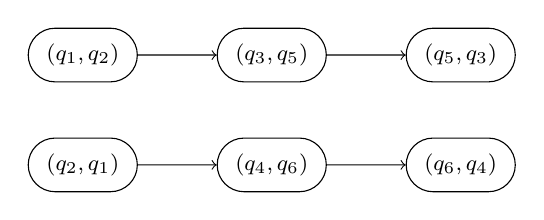
\begin{tikzpicture}[node distance=2.4cm, every node/.style={font=\footnotesize}]
                    \node[rectangular state, minimum size=0.5cm] (q1) {$(q_1, q_2)$};
                    \node[rectangular state, below=0.7cm of q1, minimum size=0.5cm] (q2) {$(q_2, q_1)$};
                    \node[rectangular state, right of=q1, minimum size=0.5cm] (q3) {$(q_3, q_5)$};
                    \node[rectangular state, right of=q3, minimum size=0.5cm] (q5) {$(q_5, q_3)$};
                    \node[rectangular state, right of=q2, minimum size=0.5cm] (q4) {$(q_4, q_6)$};
                    \node[rectangular state, right of=q4, minimum size=0.5cm] (q6) {$(q_6, q_4)$};

                    \path[->]
                            (q1) edge[above] node{} (q3)
                            (q3) edge[above] node{} (q5)
                            (q2) edge[below] node{} (q4)
                            (q4) edge[below] node{} (q6);
                    \end{tikzpicture}
                    \caption*{Supbroduct of the NPDA above.}
                \end{subfigure}
                \vspace*{1em}
                \caption{This figure illustrates a NPDA and its subproduct. The highest yield achieved through the procedure mapping based on this subproduct is 2.}
                \label{fig:trans_types}
            \end{figure}

            The following subsections provide definitions for all four types of transitions. We consider an NPDA $M = (Q, \Sigma, \Gamma_\epsilon, \delta, I, \lambda, F, \phi)$ and a procedure $P = (V, E)$ derived from a subproduct of $M$.

        \subsubsection*{Call Transition}
            A transition that enters a procedure is referred to as to call transition. The set of \textit{call transitions} for an automaton $M$ and a procedure candidate $P$ is defined as follows: $\delta_{call}(M, P) = \{(q, a, \alpha, \beta, r)\,|\,(r, \beta) \in \delta(q, a, \alpha),\\\textnormal{ where } q \in Q \setminus states(P), r \in states(P), a \in \Sigma, \alpha, \beta \in \Gamma_\epsilon\}$.

            For example, for the automaton $M$ in Figure \ref{fig:trans_types} and the maximum possible procedure candidate $P$, the set of call transitions is $\delta_{call}(M, P) = \{(s, x, \epsilon, \epsilon, q_1), (s, y,\\ \epsilon, \epsilon, q_2)\}$.

        \subsubsection*{Return Transition}
            A transition that exits a procedure is called a return transition. The set of \textit{return transitions} for an automaton $M$ and a procedure candidate $P$ is defined as: $\delta_{ret}(M, P) = \{(q, a, \alpha, \beta ,r)\,|\,(r, \beta) \in \delta(q, a, \alpha)\textnormal{, where }\\q \in states(P), r \in Q \setminus states(P), a \in \Sigma, \alpha, \beta \in \Gamma_\epsilon\}$.

            For instance, for the automaton $M$ in Figure \ref{fig:trans_types} and the maximum possible procedure candidate $P$, the set of return transitions is $\delta_{ret}(M, P) = \{(q_5, x, \epsilon, \epsilon, f), (q_6,\\ y, \epsilon, \epsilon, f)\}$.

        \subsubsection*{Procedure Transition}
            Procedure transitions are defined differently from the others. A \textit{procedure transition} uses vertices from a~procedure candidate. The set of \textit{procedure transitions} for an automaton $M$ and procedure candidate $P = (V, E)$ is $\delta_{proc}(M, P) = \{((r, r'), a, \alpha, \beta, (s, s')) \,|\,((s, \beta) \in \delta(r, a,\\ \alpha) \lor (s', \beta) \in \delta(r', a, \alpha)) \land \sigma_\epsilon(r, s) \cap \sigma_\epsilon(r', s') \neq \emptyset\}$.

            The set of procedure transitions for the automaton $M$ in Figure \ref{fig:trans_types} and the maximum procedure candidate $P$ is $\delta_{proc}(M, P) = \{((q_1, q_2), a, \epsilon, \epsilon, (q_3, q_4)), ((q_1, q_2),\\ d, \epsilon, \epsilon, (q_3, q_4)), ((q_3, q_4), b, \epsilon, \epsilon, (q_5, q_6))\}$.

        \subsubsection*{Auxiliary Transition}
            A transition that goes between two procedure states but is not procedure transition is called an auxiliary transition. The set of auxiliary transitions for the automaton $M$ and procedure candidate $P$ is defined as $\delta_{aux}(M, P) = \{(q, a, \alpha, \beta, r)\,|\,(r, \beta)\in\delta(q, a, \alpha)\textnormal{, where}\\ q, r \in states(P), a\in\Sigma, \alpha, \beta\in\Gamma_\epsilon\}\setminus T$, where the $T = \{(r,a,\alpha,\beta,s)\,|\,((r, r'), a, \alpha, \beta, (s, s')) \in \delta_{proc}(M, P)\} \cup \{(r',a, \alpha, \beta, s')\,|\,((r, r'), a, \alpha, \beta, (s, s')) \in \delta_{proc}(M, P)\}$.

            The set of auxiliary transitions for the automaton $M$ shown in Figure \ref{fig:trans_types} and the maximum possible procedure candidate $P$ is $\delta_{aux}(M, P) = \{(q_3, c, \epsilon, \epsilon, q_4)\}$.

    \subsection{Simulation}
        \textit{Simulation}\cite{Computing_simulaitons, When_simulation_meets_antichains} on a NFA $M$ is a preorder $\preceq\, \subseteq Q \times Q$. Let $a \in \Sigma$. The relation $p \preceq q$ only exists if $r \in F \implies q \in F$ and for every $r' \in \delta(r, a)$, there exists $q' \in \delta(q, a)$, which must further satisfy $r' \preceq q'$.

        The simulation relation is commonly used as an approximation of the language relation. If state $r$ is simulated by state $q$ ($r \overrightarrow{\preceq} q$), then the language of state $r$ is included in the language of state $q$ ($\overrightarrow{L}(r) \subseteq \overrightarrow{L}(q)$), but not vice versa.


\section{Minimization Techniques}
    This section lists the most commonly used minimization methods, namely: State Merging, Transition Pruning, and Saturation.

    \subsection{Strate Merging}
        Two states $p$ and $q$ can be merged into one if at least one of the following conditions is met:
        \begin{itemize}
            \item $\overleftarrow{L}(p) \subseteq \overleftarrow{L}(q) \land \overleftarrow{L}(q) \subseteq \overleftarrow{L}(p)$,
            \item $\overrightarrow{L}(p) \subseteq \overrightarrow{L}(q) \land \overrightarrow{L}(q) \subseteq \overrightarrow{L}(p)$, or
            \item $\overleftarrow{L}(p) \subseteq \overleftarrow{L}(q) \land \overrightarrow{L}(p) \subseteq \overrightarrow{L}(q)$.
        \end{itemize}

    \subsection{Transition Pruning}
        The transition $pa \rightarrow q$\footnote{Instead of $q \in \delta(p, a)$ we can write $pa \rightarrow q$.} can be removed if one of the following conditions is met:
        \begin{itemize}
            \item $\exists\, ra\rightarrow q \land \overrightarrow{L}(p) \subseteq \overrightarrow{L}(q)$,
            \item $\exists\, qa\rightarrow p \land \overleftarrow{L}(r) \subseteq \overleftarrow{L}(q)$, or
            \item $\exists\, r'a\rightarrow p' \land \overleftarrow{L}(r) \subseteq \overleftarrow{L}(r') \land \overrightarrow{L}(p) \subseteq \overrightarrow{L}(p')$.
        \end{itemize}

    \subsection{Saturation}
        The basic idea of saturation (or transition adding) is an analogy to transition pruning. The transition $pa \rightarrow q$ can be added to the automaton if one of the following conditions is met:
        \begin{itemize}
        \item $\exists\, qa\rightarrow r \land \overleftarrow{L}(p) \subseteq \overleftarrow{L}(q)$, or
        \item $\exists\, pa\rightarrow q \land \overrightarrow{L}(r) \subseteq \overrightarrow{L}(q)$.
        \end{itemize}

    \subsection{The Limitation}
        It can be seen that all minimization techniques are based on language inclusions (can be determined based on simulation). Then in the case of linear automata (without branching), or automata with the same prefix and suffix, these methods cannot be fully utilized, because in these automata, there is a minimum of states in language inclusion.

        \begin{figure}[h]
            \centering
            \captionsetup{justification=justified}
            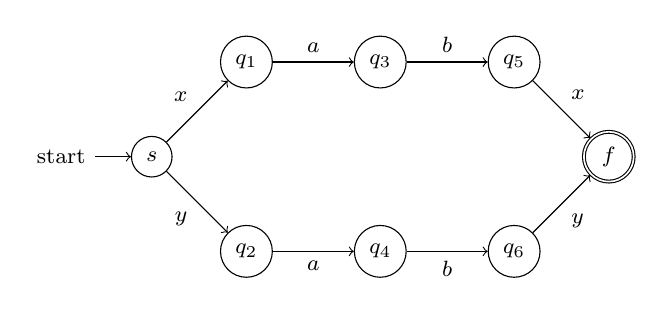
\begin{tikzpicture}[node distance=1.7cm, every node/.style={font=\footnotesize}]
              \node[state, initial, minimum size=0.5cm] (s) {$s$};
              \node[state, above right of=s, minimum size=0.5cm] (q1) {$q_1$};
              \node[state, below right of=s, minimum size=0.5cm] (q2) {$q_2$};
              \node[state, right of=q1, minimum size=0.5cm] (q3) {$q_3$};
              \node[state, right of=q3, minimum size=0.5cm] (q5) {$q_5$};
              \node[state, right of=q2, minimum size=0.5cm] (q4) {$q_4$};
              \node[state, right of=q4, minimum size=0.5cm] (q6) {$q_6$};
              \node[state, accepting, below right of=q5, minimum size=0.5cm] (f) {$f$};

            \path[->]
                      (s) edge[above left] node{$x$} (q1)
                      (s) edge[below left] node{$y$} (q2)
                      (q1) edge[above] node{$a$} (q3)
                      (q3) edge[above] node{$b$} (q5)
                      (q2) edge[below] node{$a$} (q4)
                      (q4) edge[below] node{$b$} (q6)
                      (q5) edge[above right] node{$x$} (f)
                      (q6) edge[below right] node{$y$} (f);
            \end{tikzpicture}
            \caption{An example of an automaton accepting a~word with the infix $ab$ where both the prefix and suffix must be $x$ or $y$.}
            \label{sufprefAtm}
          \end{figure}

          The illustration in Figure \ref{sufprefAtm} shows that in the automaton, no minimization based on language inclusions can be performed. However, it can be observed that the infix part of the word (unnecessarily) repeats. The main motivation for the work is the fact that in automata of this and similar types, long repeating sequences of transitions occur, which can only be represented once.

\section{Conversion of NFA to NPDA}
    This section describes the algorithm for the optimal conversion of a NFA into NPDA through the creation of procedures for similar transition sequences. In each iteration, the algorithm selects the best procedure candidate (with the highest gain) from the automaton subproduct and maps its edges to a procedure. The conversion process ends when the automaton subproduct is empty and the final automaton is reached.

    It is important to clarify what is meant by optimal conversion and how the size of the automaton is measured before discussing the algorithm in detail.

    \subsection{Conversion Efficiency}
        \label{subsec:efficiency}
        It is evident that each NFA can be transformed into a~NPDA by utilizing a single state and a stack limited to a maximum of one symbol. However, this method of transformation is not considered to be the optimal solution.

        \begin{proof}
            Let $M = (Q_M, \Sigma_M, \delta_M, I_M, F_M)$ be a NFA. For the automaton $M$ exists NPDA $N = (Q_N, \Sigma_N, \Gamma_\epsilon, \delta_N, I_N,\\ \lambda, F_N, \phi)$, such that:
            \begin{itemize}
                \item $Q_N = \{q\}$,
                \item $\Sigma_N = \Sigma_M$,
                \item $\Gamma_\epsilon = Q_M \cup \{\epsilon\}$,
                \item $\delta_N(q, a, \alpha) = (q, \beta) \iff \beta \in \delta_M(\alpha, a)$,
                \item $I_N = Q_N = \{q\}$,
                \item $\lambda(q) = I_M$,
                \item $F_N = Q_N = \{q\}$,
                \item $\phi(q) = F_M$.
            \end{itemize}
            \vspace*{-1em}
        \end{proof}

        \vspace*{-1em}
        The prior proof highlights the ease with which the number of automaton states can be reduced by using the stack to retain information of the current state of computation. Hence, the number of states holds limited significance in evaluating the optimization of the conversion. The crucial measurement for the optimal transformation of a NFA into a NPDA is the number of transitions. If the reduction  does not decrease the number of transitions, then it can be said that the conversion has not effectively reduced the size of the automaton.

        In order to attain an efficient conversion with maximal reduction in the size of the automaton, the algorithm maps only those transitions that have a~positive gain.

        \begin{figure}[!h]
            \captionsetup{justification=justified}
            \captionsetup[subfigure]{justification=centering}
            \begin{subfigure}[b]{0.485\textwidth}
                \centering
                \begin{tikzpicture}[node distance=1.7cm, every node/.style={font=\footnotesize}]
                \node[rectangular state, initial, minimum size=0.5cm] (s) {$s$};
                \node[rectangular state, above right of=s, minimum size=0.5cm] (q1) {$q_{1,2}$};
                \node[rectangular state, right of=q1, minimum size=0.5cm] (q3) {$q_{3,4}$};
                \node[rectangular state, right of=q3, minimum size=0.5cm] (q5) {$q_{5,6}$};
                \node[rectangular state, accepting, below right of=q5, minimum size=0.5cm] (f) {$f$};

                \path[->]
                        (s) edge[above left] node{$\begin{aligned}
                                                        &x, \epsilon/ q_1\\[-1mm]
                                                        &y, \epsilon/ q_2
                                                   \end{aligned}$} (q1)
                        (q1) edge[above] node{$a, \epsilon/\epsilon$} (q3)
                        (q3) edge[above] node{$b, \epsilon/\epsilon$} (q5)
                        (q5) edge[above right] node{$\begin{aligned}
                                                        &x, q_1/\epsilon\\[-1mm]
                                                        &y, q_2/\epsilon
                                                   \end{aligned}$} (f);
                \end{tikzpicture}
                \caption*{The optimally converted automaton from Figure \ref{sufprefAtm}.}
            \end{subfigure}

            \vspace*{0.5cm}

            \begin{subfigure}[b]{0.485\textwidth}
                \centering
                \begin{tikzpicture}[node distance=1.7cm, every node/.style={font=\footnotesize}]
                \node[state, initial, accepting, minimum size=0.5cm] (q) {$q$};

                \path[->]
                        (q) edge[loop right] node{$\begin{aligned}
                                                        &x, s/ q_1 &y, s/ q_2\\[-1mm]
                                                        &a, q_1/ q_3 &a, q_2/ q_4\\[-1mm]
                                                        &b, q_3/ q_5 &b, q_4/ q_6\\[-1mm]
                                                        &x, q_5/ f&y, q_6/ f
                                                    \end{aligned}$} (q);
                \end{tikzpicture}
                \caption*{The NPDA, consisting of a single state, created from the NFA in Figure \ref{sufprefAtm} representing a suboptimal conversion.}
            \end{subfigure}
            \vspace*{1em}
            \caption{The Figure illustrates the contrast between an optimal and suboptimal conversion of the NFA into a NPDA. The optimal NPDA has 5 states, 6 transitions, and utilizes 2 stack symbols, whereas the suboptimal NPDA, despite having only 1 state, has 8 transitions and requires 6 stack symbols.}
            \label{fig:optimal_red}
        \end{figure}

    \subsection{Automaton Conversion}
        The conversion of the NFA $M$ starts with transforming it into the equivalent NPDA $N$, as has been described in Section \ref{sec:NFAasNPDA}. The subproduct of automaton $N$ represents all potential procedures, where only the best candidate (with the highest gain) is selected for the mapping. The subproduct of the automaton is recalculated each time a procedure is formed. The algorithm terminates when there are no more procedure candidates (the subproduct of the automaton is empty), and the resulting automaton $N$ is returned.

        \begin{algorithm}
            \footnotesize
            \DontPrintSemicolon
            \KwIn{NFA $M = (Q_M, \Sigma_M, \delta_M, I_M, F_M)$}
            \KwOut{NPDA $N = (Q, \Sigma, \Gamma_\epsilon, \delta, I, \lambda, F, \phi)$, such that $L(N) \equiv L(M)$}

            $N \leftarrow \textit{equivalentNPDA}(M)$\tcp*{see \ref{sec:NFAasNPDA}}
            $Prod \leftarrow \textit{subproduct}(N)$\;

            \While{$Prod \neq \emptyset$}
            {
                \tcc{Find a procedure with the maximal gain.}
                $P \leftarrow argmax_{P \subseteq Prod}(G_p(P))$\;
                $N \leftarrow \textit{createProcedure}(N, Prod, P)$\;
                $N.\textit{removeStates}(\textit{states}(P))$\;
                $Prod \leftarrow \textit{subproduct}(N)$\;
            }

            \Return{$N$}

            \normalsize
            \caption{Conversion of NFA to NPDA}
            \label{alg:main}
        \end{algorithm}

    \subsection{Procedure Creation}
        Let the algorithm \ref{alg:main} selects the procedure candidate $P = (V_P, E_P)$ for mapping in automaton $M$. The following algorithm creates a new state for each pair $(r, r') \in V_P$ and assigns a stack symbol for the branches that pass through states $r$ and state $r'$ if the symbol hasn't been assigned yet in previous runs of the mapping algorithm. The function $procS: Q^M \rightarrow Q$ maps the original states $r$ and $r'$ to their respective newly created procedure states. The function $stack: Q \rightarrow 2^{\Gamma_\epsilon}$ maps each state from $states(P)$ to all possible stack symbols that can be used within a procedure state in the future. After this initiation, the procedure is constructed from all related transitions, initial states, and final states. The algorithm returns the newly created NPDA automaton $N$, where $L(M) \equiv L(N)$.

        \begin{algorithm}
            \footnotesize
            \DontPrintSemicolon
            \setcounter{AlgoLine}{0}
            \KwIn{NPDA $M = (Q^M, \Sigma, \Gamma^M_\epsilon, \delta^M, I^M, \lambda^M, F^M, \phi^M)$, subproduct $Prod = (V, E)$ of $M$, and a procedure $P = (V_P, E_P) \subseteq Prod$}
            \KwOut{NPDA $N = (Q, \Sigma, \Gamma_\epsilon, \delta, I, \lambda, F, \phi)$, such that $L(N) \equiv L(M)$}

            \vspace*{1em}
            $N \leftarrow M$\;
            \tcp{Determine stack symbols}
            $(u, v) \leftarrow root(P)$\;
            $stackU \leftarrow \{u\}$\;
            $stackV \leftarrow \{v\}$\;
            \uIf{$\gamma(u) \neq \{\epsilon\}$}
            {
                $stackU \leftarrow \gamma(u)$\;
            }\Else
            {
                $\Gamma_\epsilon \leftarrow \Gamma_\epsilon \cup \{u\}$\;
            }
            \uIf{$\gamma(v) \neq \{\epsilon\}$}
            {
                $stackV \leftarrow \gamma(v)$\;
            }\Else
            {
                $\Gamma_\epsilon \leftarrow \Gamma_\epsilon \cup \{v\}$\;
            }

            \vspace*{1em}

            $procS: Q \rightarrow Q$\;
            $stack: Q \rightarrow 2^{\Gamma_\epsilon}$\;
            \tcp{Create procedure states}
            \ForAll{$(u, v) \in V_P$}
            {
                $uv \leftarrow N.\textit{createNewState}()$\;
                $Q \leftarrow Q \cup \{uv\}$\;
                $procS(u) \leftarrow uv$\;
                $procS(v) \leftarrow uv$\;
                $stack(u) \leftarrow  stackU$\;
                $stack(v) \leftarrow stackV$\;
                $stack(uv) \leftarrow stack(u) \cup stack(v)$\;
            }
            \tcp{Map procedure}
            $N \leftarrow \textit{mapCallT}(N, \delta_{call}(Prod, P), stack, procS)$\;
            $N \leftarrow \textit{mapRetT}(N, \delta_{ret}(Prod, P), stack, procS)$\;
            $N \leftarrow \textit{mapProcT}(N, \delta_{proc}(Prod, P),stack, procS)$\;
            $N \leftarrow \textit{mapAuxT}(N, \delta_{aux}(Prod, P), stack, procS)$\;
            $N \leftarrow \textit{mapInitS}(N, P, stackU, stackV)$\;
            $N \leftarrow \textit{mapFinS}(N, P, stackU, stackV)$\;

            \Return{$N$}

            \normalsize
            \caption{createProcedure}
        \end{algorithm}

        \subsubsection*{Call Transitions}
            The algorithm mapCallT maps all transitions that enter procedure $P$. These transitions are passed to the algorithm as a set $T$. Only transitions from $T$ with a~push symbol equal to $\epsilon$ can be necessary to modify. Let $(q, a, pop, push, r)$ be a transition from $T$ where $push = \epsilon$, the $push$ symbol can be replaced with a~call symbol from $stack(r)$ if and only if $|stack(r)| = 1$, meaning that state $r$ has not been part of any procedure before. In other cases, the substitution is unnecessary as the transition $(q, a, pop, push, r)$ is already part of a~larger procedure.

            \begin{algorithm}
                \footnotesize
                \DontPrintSemicolon
                \setcounter{AlgoLine}{0}
                \KwIn{NPDA $M = (Q^M, \Sigma, \Gamma_\epsilon, \delta^M, I^M, \lambda^M, F^M, \phi^M)$, transitions $T \subseteq (Q^M \times \Sigma \times \Gamma^M_\epsilon \times \Gamma_\epsilon \times Q^M$), $stack: Q^M \rightarrow 2^{\Gamma^M_\epsilon}$ and $procS: Q^M \rightarrow Q^M$}
                \KwOut{NPDA $N = (Q, \Sigma, \Gamma_\epsilon, \delta, I, \lambda, F, \phi)$, such that $L(N) \equiv L(M)$}

                $N \leftarrow M$\;
                \ForAll{$(q, a, \alpha, \beta, r) \in T$}
                {
                    \uIf{$\alpha = \epsilon \land \beta = \epsilon \land |stack(q)| = 1$}
                    {
                        $\beta \leftarrow unpack(stack(r))$\;
                    }
                    \ElseIf{$\alpha \neq \epsilon \land \beta = \epsilon$}
                    {
                        $\beta \leftarrow unpack(stack(r))$\tcp*{$|stack(r)| = 1$}
                    }
                    $\delta(q, a, \alpha) \leftarrow \delta(q, a, \alpha) \cup \{(procS(r), \beta)\}$\;
                }

                \Return{$N$}

                \normalsize
                \caption{mapCallT}
                \label{alg:call}
            \end{algorithm}

        \subsubsection*{Return Transitions}
            \begin{algorithm}
                \footnotesize
                \DontPrintSemicolon
                \setcounter{AlgoLine}{0}
                \KwIn{NPDA $M = (Q^M, \Sigma, \Gamma^M_\epsilon, \delta^M, I^M, \lambda^M, F^M, \phi^M)$, transitions $T \subseteq (Q^M \times \Sigma \times \Gamma^M_\epsilon \times \Gamma^M_\epsilon \times Q^M$), $stack: Q^M \rightarrow 2^{\Gamma^M_\epsilon}$ and $procS: Q^M \rightarrow Q^M$}
                \KwOut{NPDA $N = (Q, \Sigma, \Gamma_\epsilon, \delta, I, \lambda, F, \phi)$, such that $L(N) \equiv L(M)$}

                $N \leftarrow M$\;
                \ForAll{$(q, a, \alpha, \beta, r) \in T$}
                {
                    \If{$\alpha = \epsilon \land \beta = \epsilon \land |stack(q)| \neq 1$}
                    {
                        \ForAll{$\alpha \in stack(q)$}
                            {
                                $\begin{aligned}\delta(procS(q), a, \epsilon) \leftarrow &\delta(procS(q), a, \alpha)\\
                                     &\cup \{(r, \alpha)\}
                                \end{aligned}$
                            }
                        \textbf{continue}\;
                    }
                    \uIf{$\alpha = \epsilon \land \beta = \epsilon \land |stack(q)| = 1$}
                    {
                        $\alpha \leftarrow unpack(stack(q))$\;
                    }\ElseIf{$\alpha = \epsilon \land \beta \neq \epsilon$}
                    {
                        $\alpha \leftarrow unpack(stack(q))$\tcp*{$|stack(q)| = 1$}
                    }
                    $\delta(procS(q), a, \alpha) \leftarrow \delta(procS(q), a, \alpha) \cup \{(r, \beta)\}$\;
                }

                \Return{$N$}

                \normalsize
                \caption{mapRetT}
            \end{algorithm}

            The mapping of return transitions that exit a procedure $P$ is analogous to the mapping of call transitions. The transitions are passed to the algorithm as a set $T$. Only transitions from $T$ with a pop symbol equal to $\epsilon$ may require modification. The modification is similar to that described in Algorithm \ref{alg:call}. However, if the transition $(q, a, \epsilon, push, r)$ occurs and $|stack(q)| > 1$, then the transition $(q, a, \alpha, push, r)$ must be mapped to the procedure for each $\alpha \in stack(q)$.

        \subsubsection*{Procedure Transitions}
            The procedure transitions are passed to the algorithm as $T \subseteq ((Q^M\times Q^M) \times \Sigma \times \Gamma^M_\epsilon \times \Gamma^M_\epsilon \times (Q^M\times Q^M))$. This set is transformed into $T' \subseteq (Q^M \times \Sigma \times \Gamma^M_\epsilon \times \Gamma^M_\epsilon \times Q^M)$ through the following process: the transition $((r, r'), a, \epsilon, \epsilon, (s, s'))$ is transformed to $(r, a, \epsilon, \epsilon, s)$ if a transition $(s, \epsilon) \in \delta^M(r, a, \epsilon)$ and an equivalent transition $(s', \epsilon) \in \delta^M(r', a, \epsilon)$ exist. If the transition is specific to states $r$ and $s$, it is transformed to $(r, a, \alpha, \alpha, s)$, for every $\alpha \in stack(r)$. Similarly, if the transition is specific to states $r'$ and $s'$.

            \begin{algorithm}
                \footnotesize
                \DontPrintSemicolon
                \setcounter{AlgoLine}{0}
                \KwIn{NPDA $M = (Q^M, \Sigma, \Gamma^M_\epsilon, \delta^M, I^M, \lambda^M, F^M, \phi^M)$, transitions $T \subseteq ((Q^M\times Q^M) \times \Sigma \times \Gamma^M_\epsilon \times \Gamma^M_\epsilon \times (Q^M\times Q^M))$, $stack: Q^M \rightarrow 2^{\Gamma^M_\epsilon}$ and $procS: Q^M \rightarrow Q^M$}
                \KwOut{NPDA $N = (Q, \Sigma, \Gamma_\epsilon, \delta, I, \lambda, F, \phi)$, such that $L(N) \equiv L(M)$}

                \tcc{Transform $T$ to $(Q^M \times \Sigma \times \Gamma^M_\epsilon \times \Gamma^M_\epsilon \times Q^M)$ format}
                $T' \leftarrow \emptyset$\;
                \ForAll{$((r, r'), a, \alpha, \beta, (s, s')) \in T$}
                {
                    \uIf{$\alpha = \epsilon \land \beta = \epsilon$}
                    {
                        \uIf{$a \in \sigma_\epsilon(r, s) \cap \sigma_\epsilon(r', s')$}
                        {
                            $T' \leftarrow T' \cup \{(r, a, \alpha, \beta, s)\}$\;
                        }\uElseIf{$a \in \sigma_\epsilon(r, s) \setminus \sigma_\epsilon(r', s')$}
                        {
                            \ForAll{$\eta \in stack(r)$}
                            {
                                $T' \leftarrow T' \cup \{(r, a, \eta, \eta, s)\}$\;
                            }
                        }\Else
                        {
                            \ForAll{$\eta \in stack(r')$}
                            {
                                $T' \leftarrow T' \cup \{(r, a, \eta, \eta, s)\}$\;
                            }
                        }
                    }\Else
                    {
                        $T' \leftarrow T' \cup \{(r, a, \alpha, \beta, s)\}$\;
                    }
                }

                $N \leftarrow M$\;
                \ForAll{$(q, a, \alpha, \beta, r) \in T'$}
                {
                    $\begin{aligned}\delta(procS(q), a, \alpha) \leftarrow &\delta(procS(q), a, \alpha)\\
                        & \cup \{(procS(r), \beta)\}
                    \end{aligned}$
                }

                \Return{$N$}

                \normalsize
                \caption{mapProcT}
            \end{algorithm}

        \subsubsection*{Auxiliary Transitions}
            All auxiliary transitions between two states of the procedure $P$ that are not classified as procedure transitions are passed to the algorithm as a set $T$. Each transition in $T$ is modified by substituting $\epsilon$ symbols with the corresponding stack symbols. Consider a transition $(q, a, \alpha, \beta, r)$. If $\alpha = \epsilon$, it is substituted with a symbol from $stack(q)$. Similarly, if $\beta = \epsilon$, it is substituted with a symbol from $stack(r)$.
        \begin{algorithm}
            \footnotesize
            \DontPrintSemicolon
            \setcounter{AlgoLine}{0}
            \KwIn{NPDA $M = (Q^M, \Sigma, \Gamma^M_\epsilon, \delta^M, I^M, \lambda^M, F^M, \phi^M)$, transitions $T \subseteq (Q^M \times \Sigma \times \Gamma^M_\epsilon \times \Gamma^M_\epsilon \times Q^M$), $stack: Q^M \rightarrow 2^{\Gamma^M_\epsilon}$ and $procS: Q^M \rightarrow Q^M$}
            \KwOut{NPDA $N = (Q, \Sigma, \Gamma_\epsilon, \delta, I, \lambda, F, \phi)$, such that $L(N) \equiv L(M)$}

            $N \leftarrow M$\;
            \ForAll{$(q, a, \alpha, \beta, r) \in T$}
            {
                \If{$\alpha = \epsilon \land \beta = \epsilon$}
                {
                    $\alpha \leftarrow unpack(stack(q))$\tcp*{$|stack(q)| = 1$}
                    $\beta \leftarrow unpack(stack(r))$\tcp*{$|stack(r)| = 1$}
                }\uElseIf{$\alpha = \epsilon \land \beta \neq \epsilon$}
                {
                    $\alpha \leftarrow unpack(stack(q))$\tcp*{$|stack(q)| = 1$}
                }\ElseIf{$\alpha \neq \epsilon \land \beta = \epsilon$}
                {
                    $\beta \leftarrow unpack(stack(r))$\tcp*{$|stack(r)| = 1$}
                }

                $\begin{aligned}\delta(procS(q), a, \alpha) \leftarrow &\delta(procS(q), a, \alpha)\\
                    & \cup \{(procS(r), \beta)\}
                \end{aligned}$
            }

            \Return{$N$}

            \normalsize
            \caption{mapAuxT}
        \end{algorithm}

        \subsubsection*{Initial States}
            The mapping of initial states into a procedure $P$ is crucial as it determines how the resulting NPDA nondeterministically puts the initial symbols from $\Gamma_\epsilon$ onto the stack according to the function $\lambda: I \rightarrow 2^{\Gamma_\epsilon}$. If the original initial state $p$ is mapped into the procedure state $s$, then the $s$ will become an initial state and will nondeterministically put the symbol from $stack(p)$ onto the stack.

        \begin{algorithm}
            \footnotesize
            \DontPrintSemicolon
            \setcounter{AlgoLine}{0}
            \KwIn{NPDA $M = (Q^M, \Sigma, \Gamma^M_\epsilon, \delta^M, I^M, \lambda^M, F^M, \phi^M)$, procedure $P = (V_P, E_P)$, and two stack symbols $stackU, stackV \in \Gamma^M_\epsilon$}
            \KwOut{NPDA $N = (Q, \Sigma, \Gamma_\epsilon, \delta, I, \lambda, F, \phi)$, such that $L(N) \equiv L(M)$}

            $N \leftarrow M$\;
            \ForAll{$(u, v) \in V_P$}
            {
                $initStackU \leftarrow \emptyset$\;
                $initStackV \leftarrow \emptyset$\;
                \If{$u \in I$}
                {
                    $initStackU \leftarrow \phi(u)$ \textbf{if} $\phi(u) \neq \{\epsilon\}$ \textbf{else} $stackU$\;
                }
                \If{$v \in I$}
                {
                    $initStackV \leftarrow \phi(v)$ \textbf{if} $\phi(v) \neq \{\epsilon\}$ \textbf{else} $stackV$\;
                }
                \If{$initStackU \cup initStackV \neq \emptyset$}
                {
                    $I \leftarrow I \cup \{uv\}$\tcc*{procedure state}
                    $\lambda(uv) \leftarrow initStackU \cup initStackV$\;
                }
            }
            \Return{$N$}

            \normalsize
            \caption{mapInitS}
        \end{algorithm}

        \subsubsection*{Final States}
            The mapping of final states into a procedure $P$ is important as it determines when the NPDA accepts the input (i.e., which symbol must be at the top of the stack) according to the function $\phi: F \rightarrow 2^{\Gamma_\epsilon}$. If the original final state $p$ is mapped into the procedure state $s$, then the $s$ becomes a final state that accepts input if the symbol from $stack(p)$ is at the top of the stack.

            \begin{algorithm}
                \footnotesize
                \DontPrintSemicolon
                \setcounter{AlgoLine}{0}
                \KwIn{NPDA $M = (Q^M, \Sigma, \Gamma^M_\epsilon, \delta^M, I^M, \lambda^M, F^M, \phi^M)$, procedure $P = (V_P, E_P)$, and two stack symbols $stackU, stackV \in \Gamma^M_\epsilon$}
                \KwOut{NPDA $N = (Q, \Sigma, \Gamma_\epsilon, \delta, I, \lambda, F, \phi)$, such that $L(N) \equiv L(M)$}

                $N \leftarrow M$\;
                \ForAll{$(u, v) \in V_P$}
                {
                    $finStackU \leftarrow \emptyset$\;
                    $finStackV \leftarrow \emptyset$\;
                    \If{$u \in I$}
                    {
                        $finStackU \leftarrow \phi(u)$ \textbf{if} $\phi(u) \neq \{\epsilon\}$ \textbf{else} $stackU$\;
                    }
                    \If{$v \in I$}
                    {
                        $finStackV \leftarrow \phi(v)$ \textbf{if} $\phi(v) \neq \{\epsilon\}$ \textbf{else} $stackV$\;
                    }
                    \If{$finStackU \cup finStackV \neq \emptyset$}
                    {
                        $F \leftarrow F \cup \{uv\}$\tcc*{procedure state}
                        $\phi(uv) \leftarrow finStackU \cup finStackV$\;
                    }
                }
                \Return{$N$}

                \normalsize
                \caption{mapFinS}
            \end{algorithm}


\section{Experimental Results}
    The reduction algorithm that transforms NFA into the equivalent NPDA was evaluated on automata from the abstract regular model checking study \cite{ARMC}, small regular expressions from the Snort database of network intrusion detection system\footnote{Available at: \url{http://snort.org}}, and large regular expressions describing protocols and attacks obtained from the L7 classifier for the Linux Netfilter framework\footnote{Available at: \url{http://netfilter.org}} and Snort.

    Prior to using the reduction approach, the input automata were simplified using the RABIT tool\footnote{Available at: \url{http://languageinclusion.org}}, which uses state merging and transition pruning based on language inclusions. For large regular expressions describing protocols and attacks containing up to millions of transitions, the approximation reduction method \cite{ApproxRed} was applied before using RABIT.

    Our approach significantly reduced the results of the RABIT tool, with a reduction of 46\% in the number of states and 13.6\% in the number of transitions for automata from regular model checking, 24.5\% in states and 16.3\% in transitions for small regular expressions, and 43.9\% in states and 36.4\% in transitions for large regular expressions.

    \subsection{Regular Model Checking}
        The effectiveness of the algorithm was evaluated on 208 automata obtained from regular model checking, with up to 6800 transitions and 1600 states. The reduce tool RABIT was first used on the automata to merge language equivalent states and eliminate redundant transitions, after which our reduction algorithm was applied. The improvement in reduction was analyzed by comparing the results with the outputs of RABIT. The following graphs demonstrate the difference in the reduction of the number of states and transitions (which is the most significant measurement as noted in Subsection \ref{subsec:efficiency}) in the automata.

        \begin{figure}[!h]
            \centering
            \captionsetup{justification=justified}
            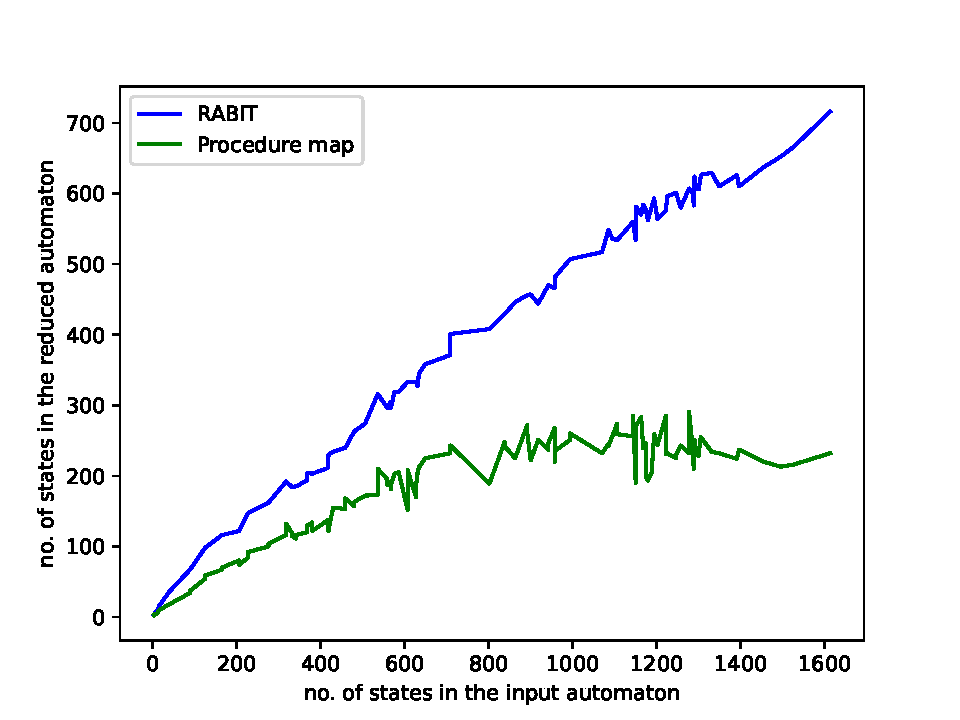
\includegraphics[width=1\linewidth]{images/armc-states.pdf}
            \caption{The graph presents a comparison of the number of states in the automata when the reduction tool RABIT is used alone or in the combination with the procedure mapping algorithm. The use of the procedure mapping algorithm resulted in a 58\% decrease in the number of states compared to the results obtained from RABIT alone.}
        \end{figure}

        \begin{figure}[!h]
            \centering
            \captionsetup{justification=justified}
            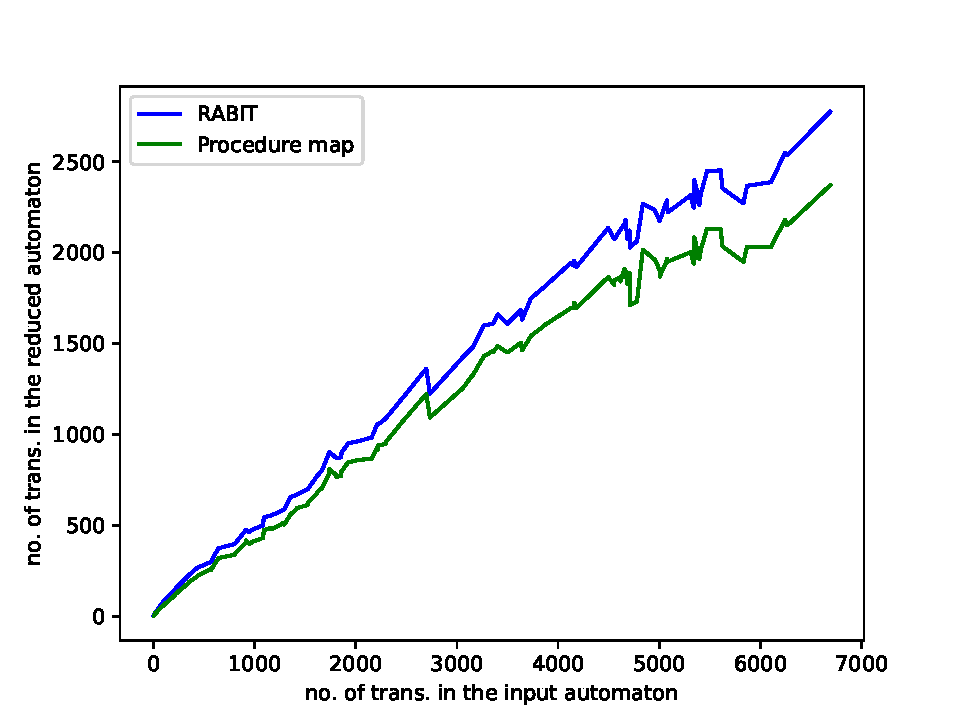
\includegraphics[width=1\linewidth]{images/armc-trans.pdf}
            \caption{The graph demonstrates a comparison of the number of transitions in the automata when the reduction tool RABIT is used individually or in conjunction with the procedure mapping algorithm. The use of the procedure mapping algorithm resulted in a 14.6\% reduction in the number of transitions compared to the results obtained from the standalone use of RABIT.}
        \end{figure}

    \subsection{Regular Expressions}
        The procedure mapping reduction is found to be more effective compared to state merging and transition pruning when applied to automata representing regular expressions. These automata often have a tree-like or even linear structure, resulting in a limited number of language equivalent states.

        The reduction was tested on 656 nearly linear automata obtained from Snort, with a maximum of 410 states and 410 transitions. The following graphs demonstrate the comparison between the reduction achieved by the RABIT tool and the reduction achieved by the procedure mapping algorithm. It is evident that the RABIT tool was unable to produce a meaningful reduction.

        \begin{figure}[!h]
            \centering
            \captionsetup{justification=justified}
            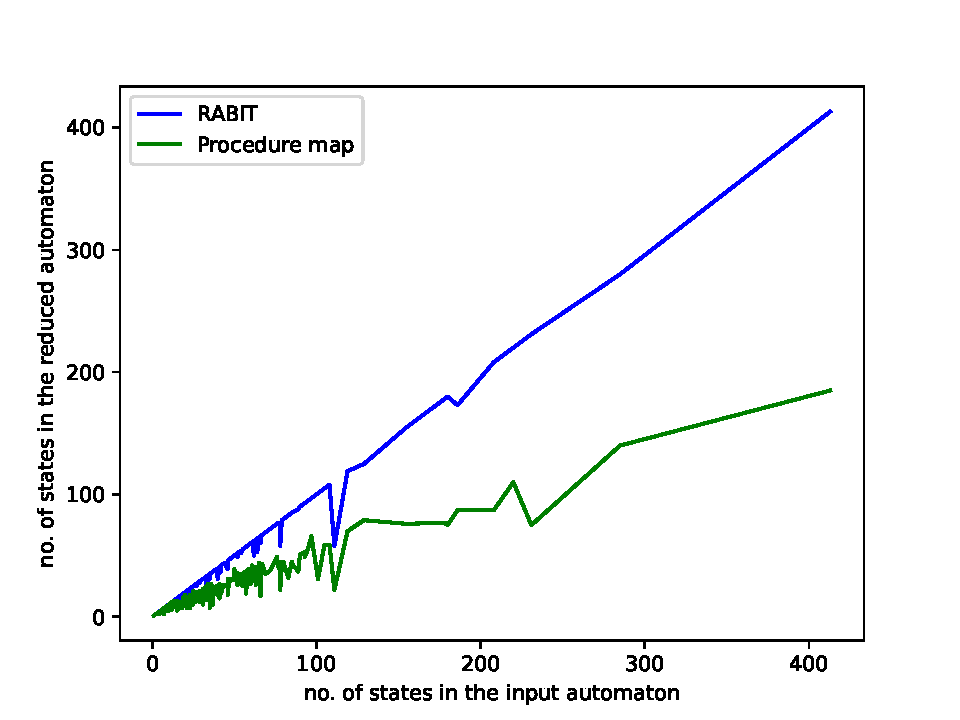
\includegraphics[width=1\linewidth]{images/stackoverflow-states.pdf}
            \caption{The reduction tool RABIT failed to achieve meaningful reduction on the input automata. In contrast, the procedure mapping reduction resulted in an average reduction of 25.9\% in the number of states of the input automata.}
        \end{figure}

        \begin{figure}[!h]
            \centering
            \captionsetup{justification=justified}
            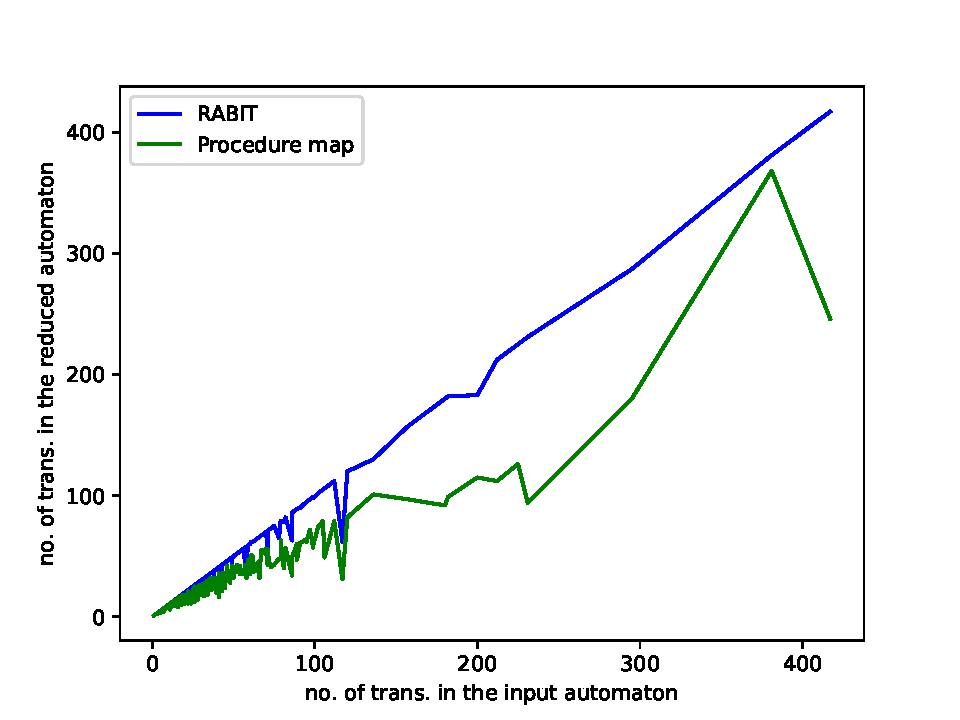
\includegraphics[width=1\linewidth]{images/stackoverflow-trans.pdf}
            \caption{The reduction tool RABIT was unsuccessful in reduction on the input automata. On the other hand, the procedure mapping reduction was able to achieve an average reduction of 16.3\% in the number of transitions of the input automata.}
        \end{figure}

    \subsection{Protocols and Attacks}
        Last but certainly not least, the procedure mapping reduction was tested on large automata representing regular expressions for protocols and attacks obtained from the L7 classifier for the Linux Netfilter framework and the Snort tool. The tested automata, \texttt{backdoor}, \texttt{pop3}, and \texttt{spyware}, were obtained from the Snort tool and provide a description of attacks on selected protocols. The \texttt{l7-all} automaton was obtained from the L7 classifier and describes attacks on a selected set of protocols.

        \begin{table}[!h]
            \centering
            \captionsetup{justification=justified}
            \footnotesize
            \begin{tabular}{|l||r|r|}
                \hline
                Automaton        	& States & Transitions\\[0.5ex]
                \hline
                \texttt{backdoor}   & 3,898  & 100,301 \\[0.5ex]
                \texttt{pop3}   	& 923	& 209,467 \\[0.5ex]
                \texttt{spyware}	& 12,809 & 279,334 \\[0.5ex]
                \texttt{l7-all}  	&7,280   &2,647,620 \\[0.5ex]
                \hline
            \end{tabular}
            \normalsize
            \caption{The sizes of the original automata representing regular expressions for protocols and attacks.}
        \end{table}

        As the automata contain hundreds of thousands, or even millions, of transitions, reducing their size is crucial before applying the RABIT tool or procedure mapping reduction. To achieve this, the approximation reduction (as described in \cite{ApproxRed}) is used. This reduction method involves a reduction in the size of the automaton at the cost of a loss in language precision. The greater the reduction ratio achieved through approximation reduction, the lower the precision.

        \begin{table}[!h]
            \centering
            \captionsetup{justification=justified}
            \scriptsize
            \begin{tabular}{|c|c|c||l|r|}
                \hline
                Automaton        	& Red. Ratio & Precision & Algorithm & States \\[0.5ex]
                \hline\hline
                \multirow{3}{*}{\texttt{backdoor}} & \multirow{3}{*}{30\%} & \multirow{3}{*}{100\%} & Approx. Red. & 1,169\\[0.5ex]
                & & & RABIT & 690\\[0.5ex]
                & & & RABIT + Proc. & 375\\[0.5ex]
                \hline
                \multirow{3}{*}{\texttt{l7-all}} & \multirow{3}{*}{30\%} & \multirow{3}{*}{35\%} & Approx. Red. & 2,184\\[0.5ex]
                & & & RABIT & 210\\[0.5ex]
                & & & RABIT + Proc. & 133\\[0.5ex]
                \hline
                \multirow{3}{*}{\texttt{pop3}} & \multirow{3}{*}{30\%} & \multirow{3}{*}{N/A} & Approx. Red. & 277\\[0.5ex]
                & & & RABIT & 77\\[0.5ex]
                & & & RABIT + Proc. & 36\\[0.5ex]
                \hline
                \multirow{6}{*}{\texttt{spyware}} & \multirow{3}{*}{30\%} & \multirow{3}{*}{100\%} & Approx. Red. & 3,843\\[0.5ex]
                & & & RABIT & 650\\[0.5ex]
                & & & RABIT + Proc. & 345\\[0.5ex]
                \cline{2-5}
                & \multirow{3}{*}{15\%} & \multirow{3}{*}{35\%} & Approx. Red. & 1,921\\[0.5ex]
                & & & RABIT & 244\\[0.5ex]
                & & & RABIT + Proc. & 154\\[0.5ex]
                \hline
            \end{tabular}
            \normalsize
            \caption{The table presents the results of the reduction for automata that have been pre-processed using the approximation reduction method. It displays the difference in the number of states in the resulting automata when the RABIT reduction tool is used alone or in the combination with the procedure mapping algorithm.}
            \label{tab:states}
        \end{table}

        After the approximation reduction, the RABIT tool was used to merge language equivalent states and remove redundant transitions, followed by the application of the procedure mapping reduction. The improvement in reduction was evaluated by comparing the results with the output of RABIT. The results obtained for different approximation reduction ratios are shown in the tables \ref{tab:states} and \ref{tab:trans}.

        \begin{table}[!h]
            \centering
            \captionsetup{justification=justified}
            \scriptsize
            \begin{tabular}{|c|c|c||l|r|}
                \hline
                Automaton        	& Red. Ratio & Precision & Algorithm & Transitions \\[0.5ex]
                \hline\hline
                \multirow{3}{*}{\texttt{backdoor}} & \multirow{3}{*}{30\%} & \multirow{3}{*}{100\%} & Approx. Red. & 31,080\\[0.5ex]
                & & & RABIT & 10,900\\[0.5ex]
                & & & RABIT + Proc. & 7,600\\[0.5ex]
                \hline
                \multirow{3}{*}{\texttt{l7-all}} & \multirow{3}{*}{30\%} & \multirow{3}{*}{35\%} & Approx. Red. & 1,230,859\\[0.5ex]
                & & & RABIT & 9,828\\[0.5ex]
                & & & RABIT + Proc. & 6,997\\[0.5ex]
                \hline
                \multirow{3}{*}{\texttt{pop3}} & \multirow{3}{*}{30\%} & \multirow{3}{*}{N/A} & Approx. Red. & 46,523\\[0.5ex]
                & & & RABIT & 8,578\\[0.5ex]
                & & & RABIT + Proc. & 4,226\\[0.5ex]
                \hline
                \multirow{6}{*}{\texttt{spyware}} & \multirow{3}{*}{30\%} & \multirow{3}{*}{100\%} & Approx. Red. & 177,302\\[0.5ex]
                & & & RABIT & 14,576\\[0.5ex]
                & & & RABIT + Proc. & 9,276\\[0.5ex]
                \cline{2-5}
                & \multirow{3}{*}{15\%} & \multirow{3}{*}{35\%} & Approx. Red. & 107,970\\[0.5ex]
                & & & RABIT & 8,408\\[0.5ex]
                & & & RABIT + Proc. & 6,395\\[0.5ex]
                \hline
            \end{tabular}
            \normalsize
            \caption{The table presents the reduction outcomes for automata that have been pre-processed with the approximation reduction method. It displays the differences in the number of transitions in the resulting automata when using the RABIT reduction tool solely or in conjunction with the procedure mapping algorithm.}
            \label{tab:trans}
        \end{table}

        The results from the tables show that the procedure mapping reduction further reduces the number of states and transitions in the resulting RABIT automaton. On average, the procedure mapping algorithm outputs 43.9\% fewer states and 36.4\% fewer transitions. The greatest reduction in states was 53.2\% for the \texttt{pop3} automaton, and the greatest reduction in transitions was 50.7\% for the same automaton.

        This experiment concluded that the procedure mapping reduction is the most efficient for the automata representing regular expressions.

\section{Conclusion}
    In this paper, a new reduction approach for NFAs is presented. Traditional minimization techniques, such as state merging and transition pruning, often result in NFAs that still contain redundant transition sequences. Our reduction algorithm replaces those redundant transition sequences in the NFA with a single procedure by transforming the input NFA into an equivalent NPDA. The information about the original branch of the automaton, entry points, and return locations is stored on the stack. This transformation results in a more efficient representation of the input NFA. Additionally, the language generated by the resulting NPDA is regular due to the limited size of the stack, which is at most one symbol.

    Our reduction algorithm was evaluated on a diverse set of automata, including 208 automata obtained from regular model checking, 656 nearly linear automata representing regular expressions obtained from Snort, and automata representing large regular expressions describing protocols and attacks obtained from the L7 classifier for the Linux Netfilter framework and the Snort tool.

    The results of our approach showed a significant reduction compared to the RABIT tool, with reductions of 46\% in the number of states and 13.6\% in the number of transitions for automata from regular model checking, 24.5\% in states and 16.3\% in transitions for small regular expressions, and 43.9\% in states and 36.4\% in transitions for large regular expressions. The greatest reduction in states was 53.2\% for the \texttt{pop3} automaton representing regular expressions for protocols and attacks, and the greatest reduction in transitions was 50.7\% for the same automaton.

    The experiments show that the minimization technique using procedure mapping is the most suitable for automata representing regular expressions due to their tree-like or almost linear structure.

\section{Future Work}
    In future research, we aim to optimize the reduction algorithm by defining a heuristic function to select the best procedure candidate based on the number of possible return transitions. The next optimization step is to substitute stack symbols to increase the number of transitions with identical pop and push symbols. A~final improvement to the algorithm is adjusting the start and end points of the procedure to reduce the number of return and call transitions.

\section{Acknowledgment}
    I would like to express my gratitude to my supervisor, Mgr. Lukáš Holík Ph.D, for his support and the time he devoted to my work on this research.

\fi

%--------------------------------------------------------
%--------------------------------------------------------
%--------------------------------------------------------
%	LITERATURA
%--------------------------------------------------------
%--------------------------------------------------------
\phantomsection
\ifczech
    \bibliographystyle{bib-styles/czplain}
\fi
\ifslovak
    \bibliographystyle{bib-styles/skplain}
\fi
\ifenglish
    \bibliographystyle{bib-styles/enplain}
\fi

\bibliography{2023-xsedym02-bib}

%--------------------------------------------------------
%--------------------------------------------------------
%--------------------------------------------------------
\end{document}
